\lecture{2}{09.08.2020}{Sistemas Hidráulicos para Controle}

\section*{Características dos Sistemas Hidráulicos}

\begin{description}
    \item[Aplicações estacionárias]:
	\begin{itemize}
	    \item Em grandes forças, pequeno porte quando comparado à acionadores elétricos;
		\item Possibilitam flexibilidade nas instalações pelas combinações de mangueiras e atuadores de baixo peso.
	\end{itemize}
    \item[Aplicações Móbeis]:
	\begin{itemize}
	    \item Adequados em condições severas;
	    \item Baixa relação peso/potência;
	    \item Disponibilidade de energia mecânica de motores de combustão.
	\end{itemize}
\end{description}

\section*{Posicionadores Hidráulicos}

Objetivam deslocar um corpo a uma posição proporcional a um sinal de entrada.

Símbolos comuns para componentes de um circuito hidráulico:

\begin{figure}[H]
    \centering
    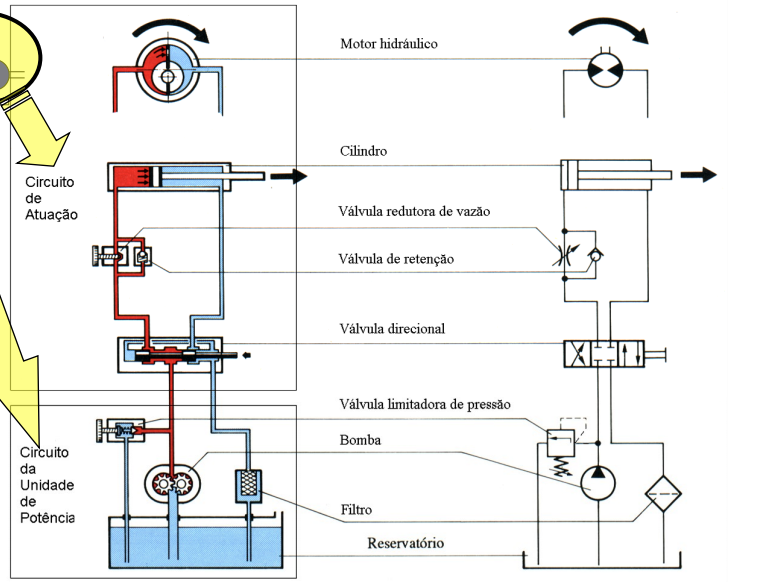
\includegraphics[width=0.8\textwidth]{figures/simbolos_circuitos.png}
    \caption{Símbolos de componentes hidráulicos comuns.}
    \label{fig:figures-simbolos_circuitos-png}
\end{figure}

\subsection*{Movimento Linear}

Pela conservação do trabalho (princípio de Pascal), utiliza-se deslocamentos diferentes em circuitos hidráulicos para se aumentar a força nas terminações.

\begin{figure}[H]
    \centering
    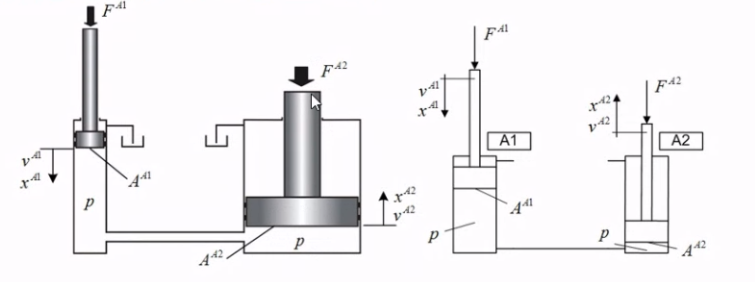
\includegraphics[width=0.8\textwidth]{figures/circuitos_hidraulicos.png}
    \caption{Atuação linear.}
    \label{fig:figures-circuito_hidraulico-png}
\end{figure}

Sabemos que a pressão é a mesma em todas as áreas em contato com o fluido, \[
p = \frac{F^{A1}}{A^{A1}} = \frac{F^{A2}}{A^{A2}}
\], então podemos aplicar a conservação do trabalho para entender a relação entre as forças e os deslocamentos resultantes \[
W = F^{A1}x^{A1} = F^{A2}x^{A2}
\].

\subsection*{Movimento Angular}

Se dá através de palhetas retrateis em um tambor descentrado, portanto, possibilitando rotação pela diferença de pressão ou da geração de diferença de pressão pela rotação.

\begin{figure}[H]
    \centering
    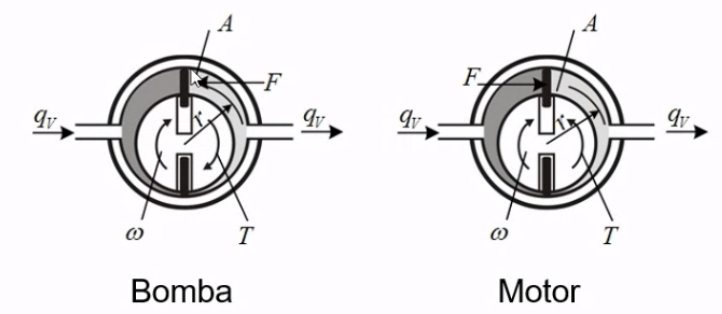
\includegraphics[width=0.8\textwidth]{figures/bomba_motor.png}
    \caption{Bomba e motor, componentes de movimento angular.}
    \label{fig:figures-bomba_motor-png}
\end{figure}

\begin{definition}
    (Deslocamento Volumétrico) Quantidade de fluido deslocado por uma bomba ou motor a cada rotação, definido como \[
	D = \frac{V}{2\pi rad} = \frac{A_{média}r2\pi}{2 \pi} = A_{média}r
    \] em que $V$ é o volume medido em metros cúbicos (m³) e pode ser calculado através da área média da palheta e o perímetro médio.
\end{definition}

Como sabemos que a pressão $p = \frac{F}{A}$ e é "propagada", temos que \[
p = \frac{F}{A} = \frac{\frac{T}{r}}{\frac{D}{r}} = \frac{T}{D}
\] o que nos propicia variar o torque em uma acoplagem motor-bomba. Além disso, analisando a variação do volume em um componente, temos que, para $\theta$ ângulo da palheta, \[
V(\theta(t)) = D\theta(t)
\] então \[
\frac{dV}{dt} = \pm D\omega(t)
\] em que o sinal depende se é uma bomba ($-$) ou atuador ($+$).

Tipos de bombas:
\begin{description}
    \item[Hidrodinâmicas] :
	\begin{itemize}
	    \item Estrutura similar a um turbo, com sucção pelo centro da hélice e descarga tangencial;
	    \item Rotor transfere energia para o fluido;
	    \item Não há separação entre sucção e descarga;
	    \item Vazão diminui drasticamente com o aumento de diferença de pressão;
	    \item Pouco uso.
	\end{itemize}
    \item[Hidrostática]:
	\begin{itemize}
	    \item Há separação entre sucção e descarga;
	    \item Fluido é seccionado e transportado para a descarga;
	    \item Pelos vazamentos decorrentes da implementação, existe uma leve queda entre a relação vazão/pressão.
	\end{itemize}
\end{description}

\subsection*{Válvulas e Bombas Fixas}

Bombas fixas fornecem pressão e vazão fixas. Portanto, se quisermos regular a velocidade de um atuador, precisamos de escape para a vazão. Para isso, utilizamos \emph{válvulas de escape}, similares à figura abaixo.

\begin{figure}[H]
    \centering
    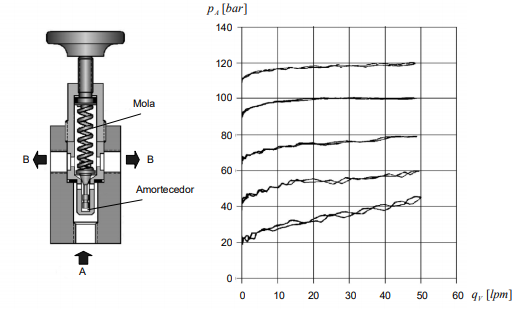
\includegraphics[width=0.8\textwidth]{figures/valvula_escape.png}
    \caption{Válvula de escape.}
    \label{fig:figures-valvula_escape-png}
\end{figure}

Para regular então a pressão para a zona de ativação da válvula de escape, utiliza-se uma \emph{válvula redutora de vazão}, que controla a área da seção transversal, portanto, controlando a diferença de pressão.

